%\pdfoutput=1
\documentclass[11pt]{article}

\usepackage[table,xcdraw]{xcolor}
\usepackage[a4paper, margin=1in]{geometry}
% \usepackage{ACL2023}
\usepackage{amsmath}
\usepackage{latexsym}
\usepackage[T1]{fontenc}

\usepackage[utf8]{inputenc}
\usepackage{fancyhdr}
\usepackage{graphicx}
\usepackage{float}
\usepackage{subfig}
\usepackage{booktabs}
\usepackage{url}
\usepackage{comment}
\usepackage{hyperref}


%%%%%%%%%%%%%%%%%%% TITLE AND AUTHORS %%%%%%%%%%%%%%%%%%%

\title{IIC3633 Aplicación de recomendación grupal de juegos de mesa utilizando metadata}

\author{\normalfont 
Eduardo Salinas | 21624453 | \texttt{esalinasbarros@uc.cl} \\
Nicolás Gutiérrez | 20203772 | \texttt{njgutierrez@uc.cl} \\
Alfonso Badilla | 20640854 | \texttt{alfonso.badilla@uc.cl} \\
% comment line below if only 3 team members
%Author 4 | SCIPER 4 | \texttt{author4@epfl.ch} \\
}

%%%%%%%%%%%%%%%%%%% PROPOSAL %%%%%%%%%%%%%%%%%%%

\begin{document}
\maketitle
\newpage

\section{Progreso en el desarrollo de la solución}

Para esta entrega hicimos el pivoteo visto en la sección 6, primero hemos entrenado varios recomendadores sencillos de baseline utilizando filtrado colaborativo, most popular, random entre otros. Para esto, utilizamos el dataset de BoardGameGeek que contiene información sobre juegos de mesa y ratings de usuarios. El dataset contiene 10 archivos diferentes, cada uno con información diferente sobre juegos de mesa. El punto de entrada fue el archivo \texttt{user\_ratings.csv} el cual consiste de 19 millones de filas. Por temas de procesamiento limitado de Google Collab (y más tarde de nuestro computador local), se utilizaron 50.000 filas para el entrenamiento inicial.

Luego, hicimos un recomendador más poderoso para este dataset, que es el que utiliza metadata. Para esto, utilizamos las categorías y mecánicas de los juegos mostrados en los otros archivos como metadata. Para esto, se utilizó la librería \texttt{fastFM} que permite entrenar modelos de factorización de matrices rápidamente. Se entrenó un modelo que recibe las categorías y mecánicas de los juegos y entrega recomendaciones para grupos de usuarios.

Además, implementamos en nuestro dataset un generador de grupos que se encarga de generar grupos de usuarios de tamaño fijo. Este generador de grupos se copió del trabajo mostrado en el paper \textit{Group Recommendation with Fast Matrix Factorization} de \textit{Yuan et al.} recuperado de su repositorio público en \href{https://github.com/barnap/group-recommenders-offline-evaluation}{github.com}.

No se logró implementar la recomendación a los grupos generados utilizando el modelo con metadata, debido a que por problemas de tiempo no se pudo hacer el ajuste necesario para que el modelo reciba los datos de entrada en el formato correcto, dado que nuestro modelo con metadata no entrega los reviews predichos, sino que entrega un orden de preferencia de los juegos (se tiene que adaptar la preferencia a un formato de predicción de rating para que funcione con las estrategias de agregación del repositorio de Group Recommendation).

En general la dirección en la que llevamos este trabajo resultó en que terminará siendo una expansión del trabajo de Yuan et al. en el sentido de que será una experimentación de qué tal funciona con un modelo con metadata.

\section{Experimentación realizada y evaluación intemredia}
A modo de experimentación se entrenaron 4 modelos de recomendación diferentes: ItemKNN, SVD, MostPopular y Random que luego se usarán como baseline.
Además, se integrá un modelo de la librería \texttt{fastFM} para crear un modelo capaz de recibir metadata y dar recomendaciones.
Para este caso particular, se entreno el modelo agregando features a items los cuales consistian en las categorias en las que se clasificaba el item a recomendar. Las features que se utilizaron 
consistian en la categoria del juego y la mecanica de este. Estos valores se convirtieron desde un flag binario a una representación vectorial como embeddings.
Se espera a futuro comparar el modelo generado con uno creado utilizando ItemKNN para ver si el modelo con metadata es capaz de dar mejores recomendaciones.
Además, queremos tratar de mejorar el modelo con metadata, revisando qué tan factible es que un usuario asigne mayor peso a ciertos embeddings que a otros, para que el modelo pueda dar recomendaciones más personalizadas para este usuario único dentro del grupo.

\section{Analisis preliminar de los resultados}
El recomendador que utiliza metadata lo comparamos con el de ItemKNN para varios grupos de usuarios de 5 integrantes. Para ellos encontramos los siguientes resultados:

\begin{table}[H]
    \centering
    \begin{tabular}{|c|c|c|c|c|}
        \hline
        \textbf{Modelo} & \textbf{Recall@10} & \textbf{Precision@10} & \textbf{NDCG@10} & \textbf{RMSE} \\ \hline
        ItemKNN & - & 0.000386 & 0.000128 & 7.13 \\ \hline
        fastFM \& metadata & 0.107 & 0.0056 & - & - \\ \hline
    \end{tabular}
    \caption{Resultados preliminares de recomendaciones para grupos}
    \label{tab:resultados_preliminares}
\end{table}

Si bien no todas las metricas estan incluidas, se puede observar que el modelo que utiliza metadata tiene un mejor recall y precision que el modelo basado en itemKNN.

En la próxima entrega deberíamos hacer cierta variación de parámetros para asegurar que sea la mejor versión de nuestro modelo con metadata.

\begin{comment}
\begin{itemize}
    \item \texttt{games.csv}: Este archivo contiene 22 atributos sobre los juegos calificados y contiene 22.000 juegos diferentes. Entre los atributos tenemos aspectos como la descripción del juego, que se podrían evaluar usando modelos de lenguaje, el año de publicación (que distribuye como se muestra en la figura \ref{fig:publishYear}), el rating promedio recibido, entre otros.
    \item \texttt{ratings\_distribution.csv}: Contiene el total de ratings en cada juego de mesa. En general estos ratings distribuyen como se ve en la figura \ref{fig:distribucionRatings}.
    \item \texttt{temes.csv}: Contiene las temáticas de cada juego como un flag binario. Las 50 más comunes se pueden ver en el gráfico de la figura \ref{fig:tematicasComunes}.
    \item \texttt{mechanics.csv}: Contiene las mecánicas del juego como un flag binario. Las 50 más comunes se pueden ver en el gráfico de la figura \ref{fig:mecanicasComunes}.
    \item \texttt{subcategories.csv}: Contiene las subcategorías de cada juego en formato flag binario.
    \item \texttt{artists\_reduced.csv}: Contiene la información sobre que artista creo cierto juego en formato flag binario. Solo se consideran artistas con mas de 3 juegos creados.
    \item \texttt{designer\_reduced.csv}: Contiene la información sobre que diseñador diseño cierto juego en formato flag binario. Solo se consideran diseñadores con mas de 3 juegos creados.
    \item \texttt{publishers\_reduced.csv}: Contiene la información de las empresas que venden dichos juegos en formato flag binario. Solo se consideran las empresas que veden mas de 3 juegos.
    
\end{itemize}


\begin{figure}
    \centering
    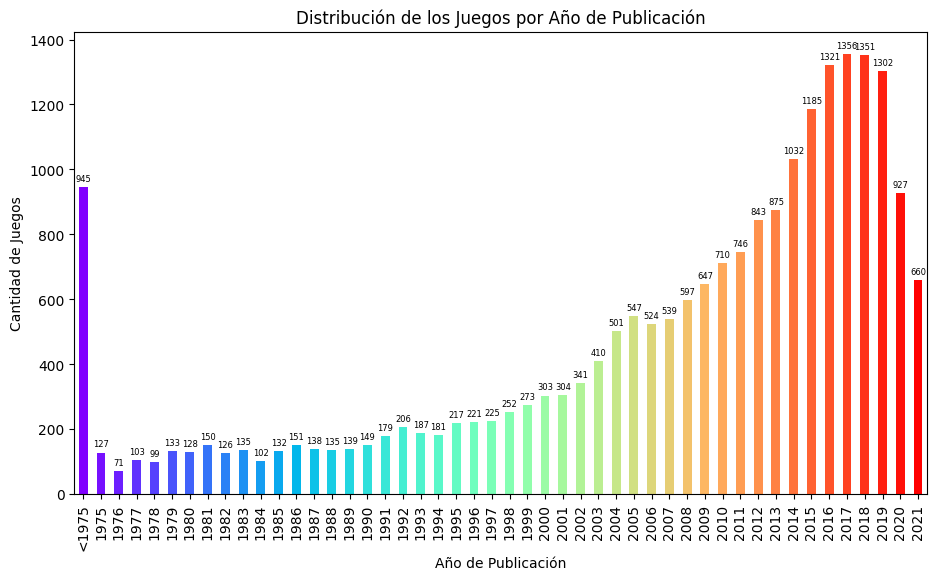
\includegraphics[width=0.8\linewidth]{publishYear.png}
    \caption{Juegos por año de publicación}
    \label{fig:publishYear}
\end{figure}

\begin{figure}[h]
    \centering
    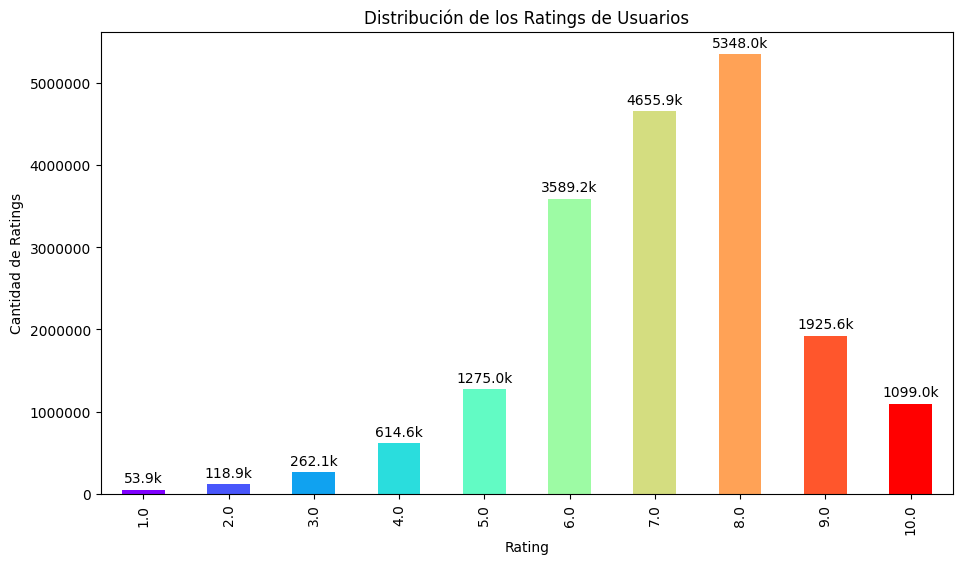
\includegraphics[width=0.8\linewidth]{distribucionRatings.png}
    \caption{Distribución de ratings de juegos}
    \label{fig:distribucionRatings}
\end{figure}

\begin{figure}[h]
    \centering
    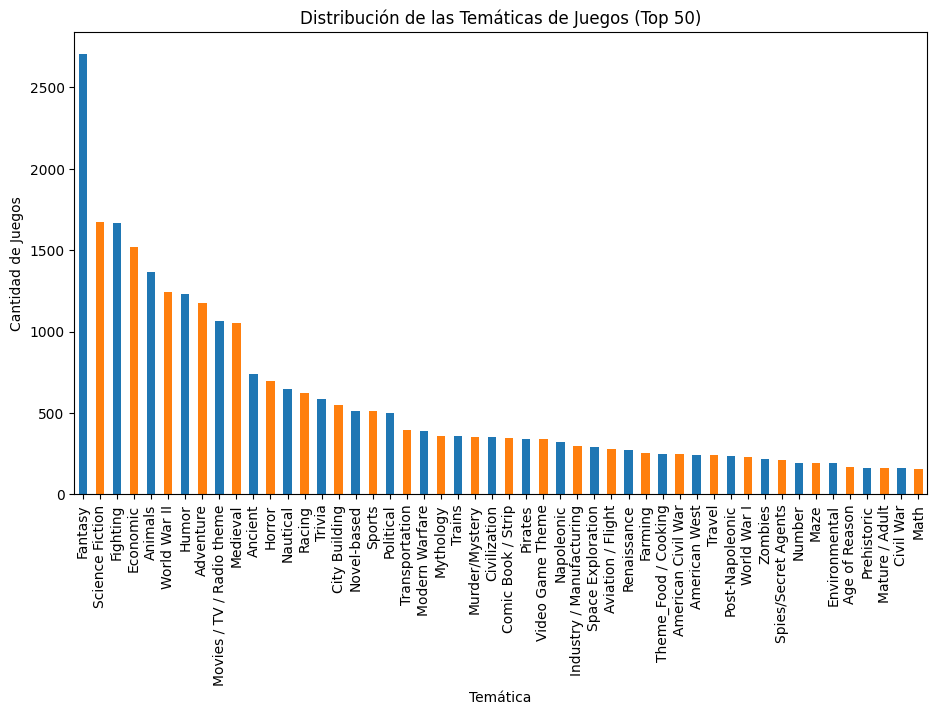
\includegraphics[width=0.8\linewidth]{tematicasComunes.png}
    \caption{Temáticas más comunes en el dataset}
    \label{fig:tematicasComunes}
\end{figure}

\begin{figure}[h]
    \centering
    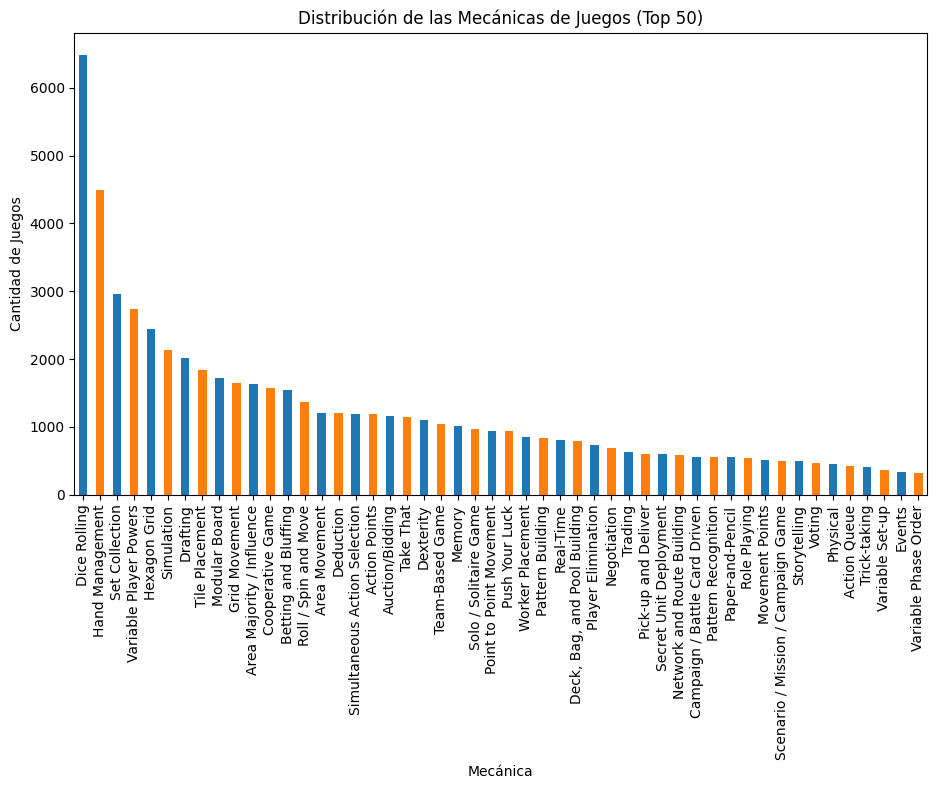
\includegraphics[width=0.8\linewidth]{mecanicasComunes.png}
    \caption{Mecánicas más comunes en el dataset}
    \label{fig:mecanicasComunes}
\end{figure}

\end{comment}

\section{Problemas identificados durante el proceso} 

Previo al pivoteo, los principales problemas que enfrentamos fueron la falta de recursos computacionales para entrenar modelos de recomendación que utilizan imágenes y la falta de experiencia en el manejo de datos de imágenes. Este problema decidimos solucionarlo cambiando la idea original del proyecto, a la cual esperamos acercarnos con recursos computacionales más poderosos.

Luego del pivoteo, los problemas que enfrentamos fueron:
\begin{itemize}
    \item Falta de obtención de metricas para comparar modelos que usan metadata.
    \item Poca flexibilidad de los modelos que utilizan metadata para recibir diferentes formatos de entrada.
    \item La capacidad limitada de cómputo de Google Colab, donde solo podíamos generar grupos con pequeñas muestras. Dado que la cantidad de 5000 grupos límite que encontramos mediante experimentación no es suficiente para hacer una evaluación robusta de los modelos, se decidió mover ese trabajo a un computador local, y se logró resolver el problema, generando en sólo 1 minuto un total de 50000 grupos los cuales se guardaron en un csv.
    \item Se espera que a futuro usar estrategias más avanzadas de creación de grupos genere que se demore más tiempo en generar los grupos, por lo que se espera que este problema se vuelva a presentar en el futuro.
\end{itemize}

\section{Revisión del plan propuesto en la etapa anterior y justificación de ajustes} 

En general, el pivoteo parece haber sido positivo, dado que gracias a este y el feedback del profesor se llegó a una idea de trabajo que busca expandir realmente el estado del arte, lo cual a efectos prácticos nos motivó y nos dio una base técnica sobre la cual construír más fácilmente.

Para la próxima entrega, planeamos terminar el recomendador grupal usando un método personalizado de simulación de ratings para poder usar las funciones de agregación del repositorio de Yuan et al.

También tendremos que solicitar feedback sobre la utilización de un repositorio público para la generación de grupos y las funciones de agregación y evaluación, ya que tenemos que compatibilizar su utilización con el código de honor.

Además, veremos si se puede hacer que cada usuario pueda elegir que cada uno de los embeddings que le corresponden tenga un peso distinto en la recomendación. Esto lo revisaremos en detalle para la entrega 3, pero puede que no sea factible o se tenga que sacar de la planeación si nos falta tiempo.

\newpage

\section{Anexo: Pivoteo en la idea original del proyecto}

El proyecto originalmente consistía en un sistema recomendador de juegos de mesa, que fuera capaz de hacer recomendaciones en base a imágenes y características descriptivas (metadata). La idea era que el sistema fuera multimodal y que pudiera recibir diferentes formatos de datos de entrada para dar recomendaciones válidas que al usuario le gustaran. 

Nosotros decidimos cambiar la idea original del proyecto por una que consideramos que podría llegar a ser más poderosa y que a nivel básico debería devolver resultados pronto. La nueva idea consiste en un sistema recomendador de juegos de mesa, que sea capaz de hacer recomendaciones para grupos en base a características descriptivas (metadata). La idea es que el sistema sea multimodal y que pueda recibir diferentes formatos de datos de entrada para dar recomendaciones válidas que al grupo de usuarios le gusten.

\section{Anexo: Actualización de propuesta}
Para hacer el pivoteo, el profesor nos pidió que hiciéramos una actualización de la propuesta a la cual debíamos agregar los siguientes puntos:
\begin{itemize}
    \item Deben agregar alrededor de 3 baselines de métodos para recomendar grupos.
    \begin{enumerate}
        \item Random es un baseline que nos permitirá saber si nuestro modelo es mejor que un modelo que recomienda juegos aleatorios. Este no debería ser difícil de superar.
        \item Most popular directamente es un baseline que podría generarnos muchos problemas superar porque cuando se recomienda a un grupo, se tiende a recomendar el juego más popular para ese tipo de grupo, y para grupos generados aleatoriamente será difícil de mejorar.
        \item ItemKNN usando la misma agregación que el modelo de metadata nos permitirá saber si el modelo de metadata mejoraría el resultado obtenido en el paper original.
    \end{enumerate}
    \item Deben actualizar la metodología de evaluación indicando métricas especificas para recomendación a grupos, no pueden hacer la misma evaluación que recomendar a individuos.
    \begin{itemize}
        \item Para la recomendación a grupos, se utilizarán las mismas métricas de evaluación que en el paper original, para verificar que nuestra expansión sea válida. Estas métricas son:
        \begin{enumerate}
            \item NDCGE, que mide la relevancia de los juegos recomendados de forma similar a NDCG para un recomendador normal.
            \item DCG, que es NDCG sin normalizar.
            \item BINARY, la métrica de evaluación binaria que se utiliza en el paper original. Esta consiste en revisar para cada recomendación, si es correcta, y luego medir la proporción de recomendaciones correctas. Luego, se aplica esta métrica según la política de agregación que se esté utilizando. 
            \item BASE, esta métrica en el paper parece ser para comparar con el modelo de recomendación base que se está utilizando. Esta métrica probablemente no la utilizaremos en el trabajo, excepto quizá para comparar con los modelos de most popular y random, si nos resulta útil.
        \end{enumerate}
    \end{itemize}
\end{itemize}

\end{document}


